\chapter{Model Validation, Preprocessing, and Responsible Evaluation}
\label{ch:validation}
\chapterguide
  {You should be able to fit and evaluate a supervised model on a held-out test set.}
  {explain cross-validation, avoid preprocessing leakage, compare thresholds, recognise overfitting, and report model limitations responsibly.}

\section{One split is one random experiment}
A single train/test split can produce an optimistic or pessimistic estimate depending on which rows happen to land in the test set. \term{Cross-validation} repeats the evaluation across several held-out folds.

\begin{utpfig}[Five-fold cross-validation]{Each fold acts as validation once while the remaining folds train the model. The final performance summary combines the held-out results.}{fig:five-fold}
\begin{tikzpicture}[x=\linewidth,y=1cm,
  foldcell/.style={draw=UTPBlue!70,fill=UTPPaleBlue,rounded corners=1mm,
    line width=0.6pt,text width=0.13\linewidth,minimum height=0.62cm,
    inner xsep=1mm,inner ysep=1mm,align=center,
    font=\scriptsize\color{UTPNavy}},
  heldout/.style={foldcell,draw=UTPTeal!80,fill=UTPPaleTeal,
    font=\scriptsize\bfseries\color{UTPNavy}},
  heading/.style={font=\scriptsize\bfseries\color{UTPNavy},inner sep=0pt}]
\node[heading,anchor=east] at (0.095,0.65) {Run};
\foreach \c in {0,...,4}{
  \pgfmathtruncatemacro{\foldnumber}{\c+1}
  \node[heading] at (0.20+\c*0.16,0.65) {Fold \foldnumber};
}
\foreach \r in {0,...,4}{
  \pgfmathtruncatemacro{\runnumber}{\r+1}
  \node[heading,anchor=east] at (0.095,-\r*0.78) {\runnumber};
  \foreach \c in {0,...,4}{
    \ifnum\r=\c
      \node[heldout] at (0.20+\c*0.16,-\r*0.78) {Validate};
    \else
      \node[foldcell] at (0.20+\c*0.16,-\r*0.78) {Train};
    \fi
  }
}
\node[font=\scriptsize\color{UTPMuted},align=center,
  text width=0.86\linewidth] at (0.50,-3.85)
  {Each run uses four training folds and one held-out validation fold.};
\end{tikzpicture}
\end{utpfig}


\begin{utpfig}[Cross-validation reveals split variation]{Each bar is held-out accuracy from a different fold of the same five-fold procedure. The variation is part of the uncertainty in generalisation performance.}{fig:validation-fold-variation}
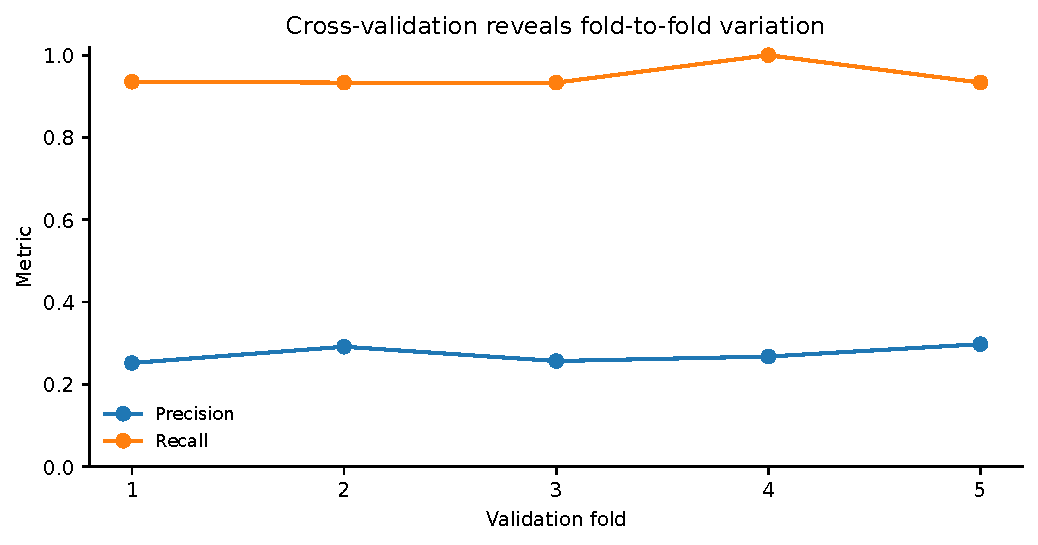
\includegraphics[width=0.79\linewidth]{figures/validation_fold_variation.pdf}
\end{utpfig}

\section{Cross-validation estimates a process, not one final model}
In $k$-fold cross-validation, $k$ temporary models are fitted to estimate how the training procedure generalises. After model choices are fixed, a final model can be refit on all available training data. The fold models are therefore evaluation instruments rather than necessarily the models that will be deployed.

Stratification is useful for classification because it keeps class proportions more consistent across folds. Grouped cross-validation is needed when observations from the same entity must stay together, such as multiple visits from one patient. Time-series data often require forward-chaining splits rather than random folds because future observations must not train models evaluated on the past.


\section{Preprocessing is learned from data}
Centering, scaling, imputation, feature selection, and encoding all estimate information from data. Therefore they belong inside the training process.

Correct order:
\begin{utpsteps}
  \item Split training and validation/test observations.
  \item Estimate preprocessing parameters from training observations only.
  \item Apply those fixed parameters to validation/test observations.
  \item Fit the model on processed training data and evaluate on processed held-out data.
\end{utpsteps}


\begin{utpfig}[Correct versus leaky preprocessing]{Any step that estimates information from data must be fitted inside the training portion of each fold. The validation rows receive parameters learned elsewhere; they do not help create them.}{fig:validation-pipeline}
\begin{tikzpicture}[x=\linewidth,y=1cm,
  card/.style={draw=UTPBlue!70,fill=UTPPaleBlue,rounded corners=1.5mm,
    line width=0.6pt,text width=0.26\linewidth,minimum height=1.45cm,
    inner xsep=2.5mm,inner ysep=2mm,align=center,
    font=\scriptsize\color{UTPNavy}},
  warning/.style={card,draw=UTPRed!80,fill=UTPPaleRed},
  flow/.style={-{Stealth[length=2mm,width=1.5mm]},
    line width=0.8pt,draw=UTPTeal,rounded corners=1.5mm},
  heading/.style={font=\scriptsize\bfseries\color{UTPNavy},anchor=west}]
\node[heading,text=UTPTeal!85!black] at (-0.145,1.1)
  {Correct: learn preprocessing from training rows only};
\node[card] (tr) at (0,0) {\textbf{Training fold}\\[4pt]
  Training observations\\only};
\node[card] (fit) at (0.335,0) {\textbf{Fit preprocessing}\\[4pt]
  Imputer, scaler,\\and feature selector};
\node[card,draw=UTPOrange!80,fill=UTPPaleOrange] (va) at (0.335,-1.8)
  {\textbf{Validation fold}\\[4pt]
   Held-out observations\\Never used for fitting};
\node[card,draw=UTPTeal!80,fill=UTPPaleTeal] (ev) at (0.670,0)
  {\textbf{Transform / evaluate}\\[4pt]
   Apply fixed training rules\\to held-out data};
\draw[flow] (tr.east) -- (fit.west);
\draw[flow] (fit.east) -- (ev.west);
\draw[flow] (va.east) -- (0.670,-1.8) -- (ev.south);
\draw[UTPMuted!35,line width=0.5pt] (-0.145,-2.9) -- (0.815,-2.9);
\node[heading,text=UTPRed!85!black] at (-0.145,-3.3)
  {Leaky: validation rows influence preprocessing};
\node[warning] (all) at (0,-4.4) {\textbf{All observations}\\[4pt]
  Training and validation\\rows combined};
\node[warning] (leakyfit) at (0.335,-4.4) {\textbf{Fit preprocessing}\\[4pt]
  Learn parameters\\from all rows};
\node[warning] (split) at (0.670,-4.4) {\textbf{Split / validate}\\[4pt]
  Held-out information\\has already leaked};
\draw[flow,draw=UTPRed!80] (all.east) -- (leakyfit.west);
\draw[flow,draw=UTPRed!80] (leakyfit.east) -- (split.west);
\end{tikzpicture}
\end{utpfig}

\begin{pitfall}
Scaling the full dataset before cross-validation lets each validation fold influence its own preprocessing. The leakage may be small in some datasets, but the evaluation principle is still broken.
\end{pitfall}

\section{Standardisation aligns feature scales}
For feature \(x\), standardisation uses
\[
z=\frac{x-\mu_{train}}{\sigma_{train}}.
\]
This is important for distance-based and regularised methods. Tree-based models are much less sensitive to monotonic scaling, which is why preprocessing should match the algorithm rather than be applied ritualistically.


\begin{utpfig}[Why scaling changes geometry]{Raw features can have completely different numerical ranges. Standardisation places them in standard-deviation units, which matters when distances or coefficient penalties compare features directly.}{fig:validation-scaling}
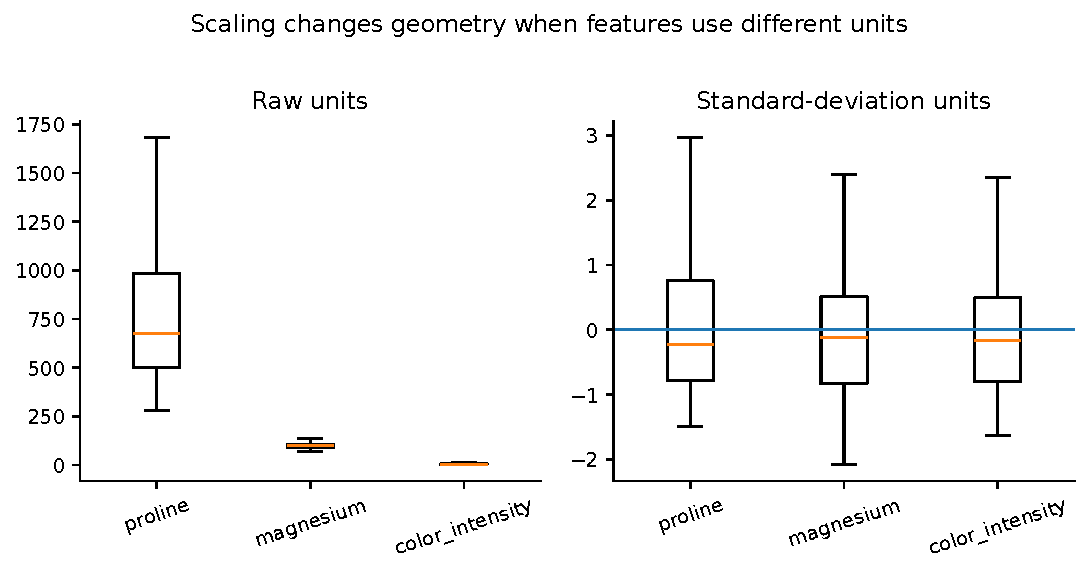
\includegraphics[width=0.92\linewidth]{figures/validation_scaling.pdf}
\end{utpfig}

\begin{utpfig}[Scaling does not make distributions identical]{After standardisation the selected features share center and scale units, but their shapes remain different. Preprocessing changes representation; it does not make the data Gaussian or remove outliers.}{fig:validation-scaled-shapes}
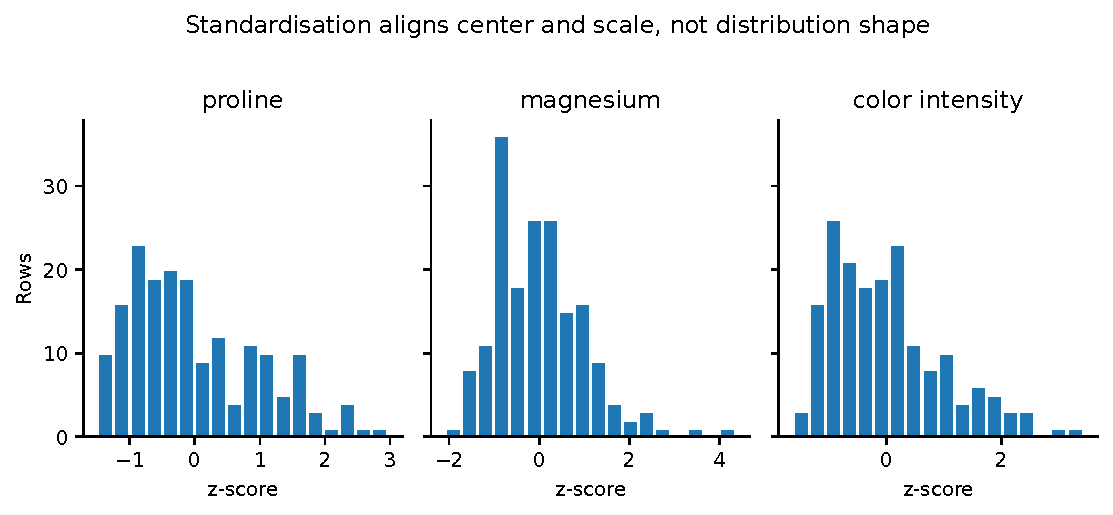
\includegraphics[width=0.80\linewidth]{figures/validation_scaled_distributions.pdf}
\end{utpfig}

\section{Hyperparameter tuning needs its own validation logic}
When cross-validation is used repeatedly to choose model complexity, features, or hyperparameters, the chosen configuration can become optimistic with respect to those same folds. A separate final test set or nested cross-validation provides a cleaner estimate of performance after tuning.

This principle generalises: any choice influenced by evaluation data---including threshold selection, feature selection, and architecture choice---has consumed some information from those data.


\section{Overfitting is a gap between fit and generalisation}
Overfitting occurs when a model captures training-specific noise or idiosyncrasy. Symptoms include excellent training performance with substantially poorer held-out performance and unstable results across folds.

\section{Thresholds, metrics, and stakeholder costs}
Different thresholds produce different confusion matrices. Model evaluation should include the metrics relevant to the actual action: detecting positives, avoiding false alarms, controlling workload, or balancing costs.


\section{Report the distribution of performance, not only the mean}
A mean cross-validation score can hide instability. Report fold scores, their spread, and any unusually weak fold. If performance depends strongly on one split, investigate whether data scarcity, subgroup imbalance, temporal drift, or duplicated entities are responsible.

\section{Subgroup evaluation needs careful denominators}
When performance is compared across groups, show group sample sizes and uncertainty as well as point metrics. A large difference in estimated error rates can be mostly sampling noise when a subgroup is small. Conversely, a good overall score can hide systematic failure in an important subgroup.


\section{Responsible evaluation goes beyond a single metric}
Check performance by meaningful subgroups when appropriate, report data provenance and exclusions, disclose uncertainty, and distinguish a teaching exercise from a deployable system. Protected or sensitive attributes require particularly careful governance and fairness analysis.

\begin{keyidea}
A model report should make failure visible: where the data came from, what preprocessing was learned, how validation was performed, which errors remain, and where the model should not be used.
\end{keyidea}

\begin{workedexample}
Lab 9 estimates scaling parameters separately inside each fold before fitting logistic regression. This small implementation detail is a core scientific principle: held-out data must remain genuinely held out.
\end{workedexample}

\begin{quickcheck}
\begin{enumerate}
  \item What does cross-validation improve compared with one random split?
  \item Which data should determine the scaling mean and standard deviation?
  \item Name one symptom of overfitting.
  \item Why might two stakeholders choose different classification thresholds for the same model?
\end{enumerate}
\end{quickcheck}

\section{Worked validation problem: rare-event fraud detection}

Credit-card fraud is a classic example of why validation metrics must match the data-generating problem. In the bundled 10,000-transaction file, only 151 records are labelled fraud---a prevalence of 1.51\%.

\begin{utpfig}[Rare classes make accuracy deceptive]{A classifier that predicts every transaction as legitimate would already achieve 98.49\% accuracy. The right panel shows that some features nevertheless differ sharply between fraud and legitimate transactions.}{fig:val-fraud-imbalance}
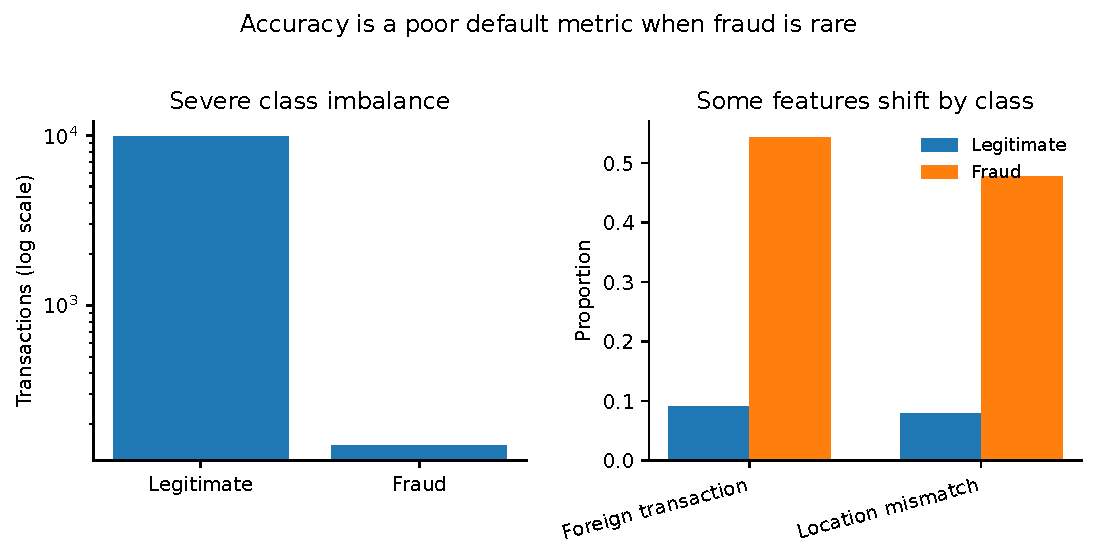
\includegraphics[width=0.90\linewidth]{figures/validation_fraud_imbalance.pdf}
\end{utpfig}

This is why precision, recall/sensitivity, specificity, false-positive rate, and threshold choice must be considered together. The best operating point depends on the relative cost of interrupting a legitimate customer versus missing a fraudulent transaction.

\begin{utpfig}[A threshold converts probabilities into operational decisions]{Changing the decision threshold moves the model along a precision--recall trade-off. Validation should compare thresholds on held-out data rather than selecting a threshold from training performance.}{fig:val-fraud-threshold}
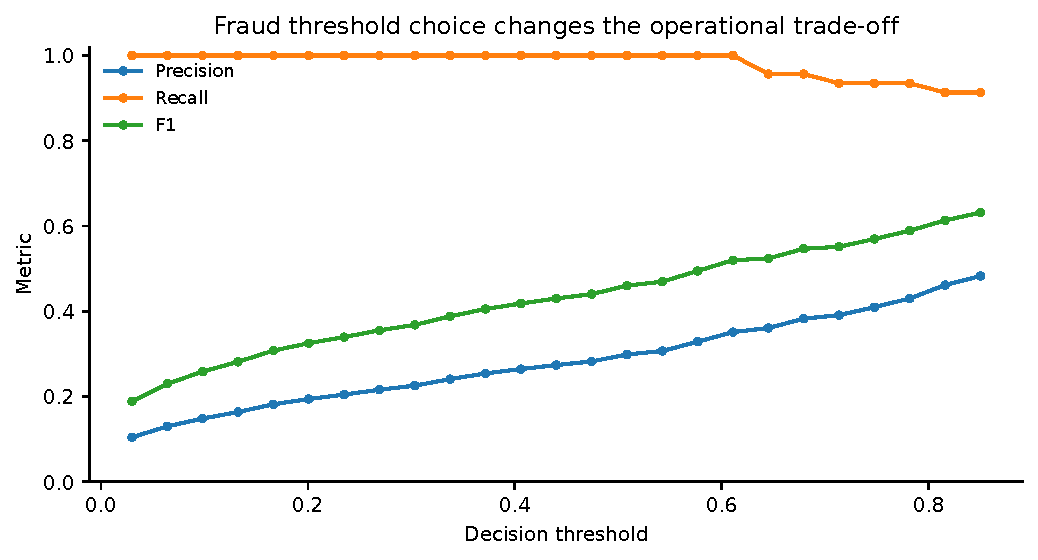
\includegraphics[width=0.82\linewidth]{figures/validation_fraud_thresholds.pdf}
\end{utpfig}

Fraud examples also make preprocessing leakage easier to understand. If scaling parameters, category encodings, resampling rules, or threshold choices are tuned using the full dataset before cross-validation, information from validation folds has influenced the training pipeline even if the final model never directly sees their labels.


\section{Calibration is a validation target when probabilities drive action}

A classifier can rank cases well while producing probabilities that are systematically too high or too low. This distinction matters when a probability is used for triage, pricing, resource allocation, or threshold selection. Calibration compares predicted probability with observed event frequency among cases receiving similar scores.

\begin{utpfig}[Heart-disease probability calibration on held-out data]{Points near the diagonal indicate agreement between predicted probability and observed positive frequency within score bins. Departures from the diagonal are a reason to investigate calibration, sample size, model specification, or distribution shift.}{fig:validation-heart-calibration}
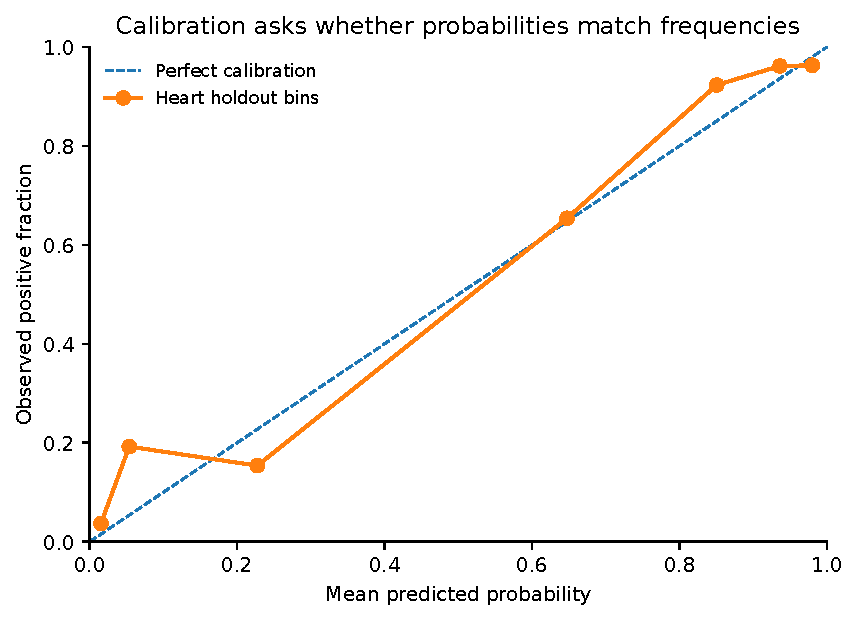
\includegraphics[width=0.68\linewidth]{figures/validation_heart_calibration.pdf}
\end{utpfig}

Calibration should be estimated on data that did not fit the model. If a separate calibration method is learned, it needs its own validation discipline as well. A well-calibrated probability is still not a causal probability, and good calibration in one population does not guarantee calibration after deployment conditions change.

\labsection{9}{Validate an imbalanced classifier without leakage}{sec:lab09}

\begin{labproject}{Validation and preprocessing: evaluate the process, not one lucky split}
\textbf{Coverage.} Chapter~\ref{ch:validation}.\\
\textbf{Goal.} You should be able to construct stratified folds, prevent preprocessing leakage, compare thresholds across folds, quantify metric variability, and distinguish discrimination from calibration.\\
\textbf{Datasets.} \texttt{credit\_card\_fraud\_dataset.csv}; Heart Failure is used for a calibration extension.\\
\textbf{Scenario.} Fraud is rare, so a superficially high accuracy can be operationally useless. You must evaluate a complete modelling process with stratified cross-validation, fold-local preprocessing, and threshold-sensitive metrics.

\textbf{Core workflow.}
\begin{enumerate}
  \item \textbf{Measure the class imbalance.} Report fraud prevalence and the accuracy of an ``always legitimate'' classifier. Treat this as the minimum baseline any useful model must beat.
  \item \textbf{Create stratified folds.} Build five folds that each contain fraud and legitimate transactions. Report the class count in every fold.
  \item \textbf{Keep preprocessing inside the fold.} For each validation fold, estimate scaling parameters from the corresponding training folds only, then apply those parameters to validation data.
  \item \textbf{Fit and retain probabilities.} Train logistic regression inside each fold and store validation probabilities so the same predictions can be evaluated at multiple thresholds.
  \item \textbf{Evaluate decision thresholds.} Compare 0.10, 0.25, and 0.50 using accuracy, precision, recall, and specificity. Include false-positive and false-negative counts where useful.
  \item \textbf{Report variability.} Summarise both the mean and fold-to-fold spread of the metrics. Identify whether recall is stable enough to support a reliable operational claim.
  \item \textbf{Choose a threshold from a stated cost.} Define a hypothetical relative cost for missed fraud versus false alarms, then select the threshold that best reflects that priority. Make clear that the cost assumption is external to the model.
\end{enumerate}

\textbf{Calibration extension.} Reuse the Heart Failure modelling workflow, bin held-out predicted probabilities, and compare mean predicted probability with observed event rate. Explain why a model can rank cases well yet still produce poorly calibrated probabilities.

\tcbbreak
\lstinputlisting[style=utpr]{all_experiments/lab09_validation.R}
\begin{verification}
\textbf{Required evidence.} Submit the majority-class baseline, five-fold metric summary, one variability result, and a threshold recommendation tied to an explicit error-cost assumption. Include one sentence identifying where leakage would occur if global scaling were applied before cross-validation.

\textbf{Professional standard.} Validation must reproduce the full future prediction process. Any transformation learned from all records before validation contaminates the estimate of generalisation performance.
\end{verification}
\end{labproject}

